\chapter{Methodology} \sloppy
\section{Software Development Approach}
 Agile is an iterative process-based approach to software development. In the Agile process model, work is broken down into more manageable, smaller iterations without requiring a lot of long-term planning. The requirements and scope of the project are determined early on, and the number, length, and scope of each iteration are preplanned. Each iteration is considered as a short time ``frame'' in the Agile process model, which lasts for a few weeks. In each iteration, teams move through the phases of the software development life cycle, which include planning, requirements analysis, design, coding, testing, and demonstration of a working product for client review. Agile places a significant value on flexibility, teamwork, and regular client feedback.\\
\begin{figure}[H]
    \centering
    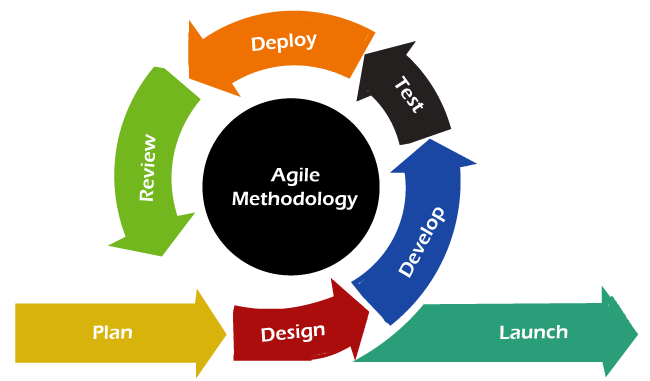
\includegraphics[width=80mm]{./img/agile.png}
    \caption*{\small{\textit{Source: https://www.javatpoint.com/agile-vs-waterfall-model}}}
    \caption{Agile Model}
\end{figure}
The main reason for which  we choose this development process:
\begin{enumerate}[noitemsep] %label=\Roman*.]
\item Very quick,flexible and efficient.
\item Risk minimization.
\item Projects are split into sprints for better management and productivity.
\item Through iterative testing and sprints, the final product contains less bugs. 
\item Development period for applications is reduced.
\end{enumerate}
\section{Data Collection} 
We have gathered data from the IStego100K dataset\cite{7}, a comprehensive collection of images for steganalysis research. The training images in IStego100K were collected from Unsplash\footnote{\url{https://unsplash.com/}}, a copyright free photography website. This dataset consits 200,000 JPEG images, divided into two main categories: "Stego" and "Cover," each containing 100,000 images. The "Stego" subset consists of images where the original cover images from the dataset have been modified to hide information. Each steganographic image is randomly steganized with three widely used image steganography algorithms (J-uniward\cite{22} ,NSF5\cite{17} and UERD\cite{13}) with a random embedding rate (0.1-0.4bpac). This diversity makes the dataset particularly valuable for developing models capable of detecting hidden data across various embedding techniques and makes dataset universal. Conversely, the "Cover" subset consists of unaltered images, serving as the baseline for comparison.\\
The images in the dataset are standardized to 1024x1024 pixels in RGB format, with each image assigned random quality factors ranging from 75 to 95. Additionally, the payload for embedding is randomly distributed within the range of 0.1 to 0.4 bits per coefficient (bpac).[0.10 bpac means that for every  cofficient in the DCT domain of the cover image, 0.10 bits of secret data are hidden on average.]\\
There are alternative datasets for steganalysis, such as BOSSbase 1.01 and BURSTbase. However, these datasets utilize images in .pgm format and we felt difficult to work with images in .pgm formatt. We preferred for the IStego100K dataset due to its utilization of .jpg format. Additionally, while the former datasets employ a single steganographic algorithm for embedding information, IStego100K employs three different algorithms, enhancing its diversity and utility for research purposes. Downloading the IStego100K dataset was much easier because it was available on Google Drive, whereas the other datasets were harder to find and access. Additionally, the information provided about the IStego100K dataset was clearer compared to the limited details available for the other datasets. Another advantage of IStego100K is that it's newer, which suggests it might be more up-to-date and relevant for current research compared to the older datasets. 


\section{Pre-feature Space}
The pre feature space is the space before the feature extraction process which involves various processes such as normalization, noise reduction or other process to enhance the quality of the data before feature extraction.
The images was changed or modified as necessary in order to prepare them for feature extraction process. The feature extraction process we were to perform was CC-C300 which took features from only on channel from the RGB so, to ensure that all the information from image is considered we turned the colored image into gray scaled image which lets go off all its other information and holds most or all of its information in the luminance channel.
\section{Feature extraction}
\subsection{JPEG Coefficient Analysis}
In the initial step, the JPEG coefficients for each $8 \times 8$ block are computed, denoted as $D(i,j)(k,l)$, representing the $(k, l)$ coefficient in the $i, j$ block. Here, $k, l = 0, 1, 2, ...7$, $i = 1, 2, 3, ..., 8(M/8)$, and $j = 1, 2, 3, ..., 8(N/8)$, with $M \times N$ as image dimensions. Subsequently, the coefficients undergo truncation to simplify complexity, ensuring the quantized DCT or JPEG coefficients are centered around 0.

The distribution of the differences between JPEG coefficients exhibits a Laplacian-like pattern, with most values close to zero. Truncation is applied to all available JPEG coefficients, expressed as $D(i,j)(k,l) \leftarrow \text{trunc}_T(D(i,j)(k,l))$, where $\text{trunc}_T(x) = x$ for $x \in [-T, T]$.
\[
    P(\Delta i, \Delta j,k_1,l_1,k_2,l_2)=\left \{ \left [ D^{(i,j)}_{k_1l_1},D^{(i+\Delta i,j+\Delta j)}_{k_2l_2} \right ] \vert i=1,...,N^{(i)}, j=1,...,N^{(j)})\right \}
\]

Following truncation, the values are processed to form pairs, and a co-occurrence matrix is computed based on the condition $|\triangle(i)| + |\triangle(j)| + |k_1 - k_2| + |l_1 - l_2| > 0$, ensuring distinct coefficients are utilized. Here, $\triangle(i) = i_1 - i_2$ and $\triangle(j) = j_1 - j_2$. The resulting co-occurrence matrix is derived from the truncation process, generating a transition probability matrix with a dimensionality of $(2T + 1) \times (2T + 1)$. For instance, if $T = 4$, the co-occurrence matrix takes on a dimension of 81 for every pair of DCT modes denoted by $(\triangle(i), \triangle(j), k_1, l_1, k_2, l_2)$.
\[
    Cst = \frac{1}{N^{(i)}N^{(j)}} \sum_{i=1}^{N^{(i)}} \sum_{j=1}^{N^{(j)}} \left[ a, b \right] \in P (\Delta i, \Delta j, k1, l1, k2, l2) | a = s, b = t
\]

\subsection{Truncation}
The co-occurrence matrix is calculated between each pair as depicted in img 2. The truncation process yields a transition probability matrix with a dimensionality of $(2T + 1) \times (2T + 1)$. When the threshold value ($T$) is set to 1, considering elements within the range $\{-1, 0, 1\}$, it results in a transition probability matrix with a dimensionality of $3 \times 3$.

Let's denote the states as -1, 0, and 1, and assume a hypothetical transition probability matrix $P$:
\[
    P = \begin{bmatrix}
        p_{-1,-1} & p_{0,-1} & p_{1,-1} \\
        p_{-1,0}  & p_{0,0}  & p_{1,0}  \\
        p_{-1,1}  & p_{0,1}  & p_{1,1}
    \end{bmatrix}
\]

In this matrix:

- $p_{-1,-1}$ represents the probability of transitioning from state -1 to state -1.
- $p_{-1,0}$ represents the probability of transitioning from state -1 to state 0.
- Similarly, the other entries follow the same pattern for transitions between states 0 and 1.

The truncation value $T$ is set to 4, resulting in a co-occurrence matrix of dimension 81 for every pair of DCT modes represented by $(\triangle(i), \triangle(j), k_1, l_1, k_2, l_2)$.

Initially, all possible DCT mode pairs are sorted based on their importance, and co-occurrences are then formed from the most important to the least important ones. As a measure of importance, mutual information (MI) is computed over a sufficiently large set of randomly selected DCT coefficient pairs from those two modes, using the \texttt{mutual\_info\_score(mode1, mode2)} where \texttt{mode1} and \texttt{mode2} are selected randomly.

\subsection.{Feature Set Creation}

The top $N$ concatenated co-occurrence matrices, denoted as $CN$, yield a dimension of $N \times 81$. After Cartesian calibration, the dimensionality of what we denote as $CC-CN$ doubles to $2 \times N \times 81$. Choosing $N$ as 300, we have $CC-C300$ with a dimensionality of $2 \times 300 \times 81 = 48,600$ for each image, irrespective of image dimensionality.

For the concatenated matrix, let
\[
    C_1 = \begin{bmatrix} 1 & 2 & 3 \\ 4 & 5 & 6 \\ 7 & 8 & 9 \end{bmatrix}, \quad
    C_2 = \begin{bmatrix} 9 & 8 & 7 \\ 6 & 5 & 4 \\ 3 & 2 & 1 \end{bmatrix}, \quad
    C_3 = \begin{bmatrix} 0 & 1 & 0 \\ 1 & 1 & 1 \\ 0 & 1 & 0 \end{bmatrix}.
\]

For $CC-C2$, the importance of each co-occurrence matrix is determined by mutual information (MI). If $C_1$ and $C_2$ are of highest importance, a new matrix is formed by concatenating $C_1$ and $C_2$.

\[
    C = \begin{bmatrix} 1 & 2 & 3 \\ 4 & 5 & 6 \\ 7 & 8 & 9 \\ 9 & 8 & 7 \\ 6 & 5 & 4 \\ 3 & 2 & 1 \end{bmatrix},
\]

where the dimension is $2 \times 3 \times 3 = 18$.

For mutual information (MI) to calculate the importance of co-occurrence, entropy and conditional entropy for each feature are calculated. The mutual information is then computed as the difference between entropy and conditional entropy for each feature, given by \text{mutual\_info\_score}(mode1, mode2).\
\begin{figure}[H]
    \centering
    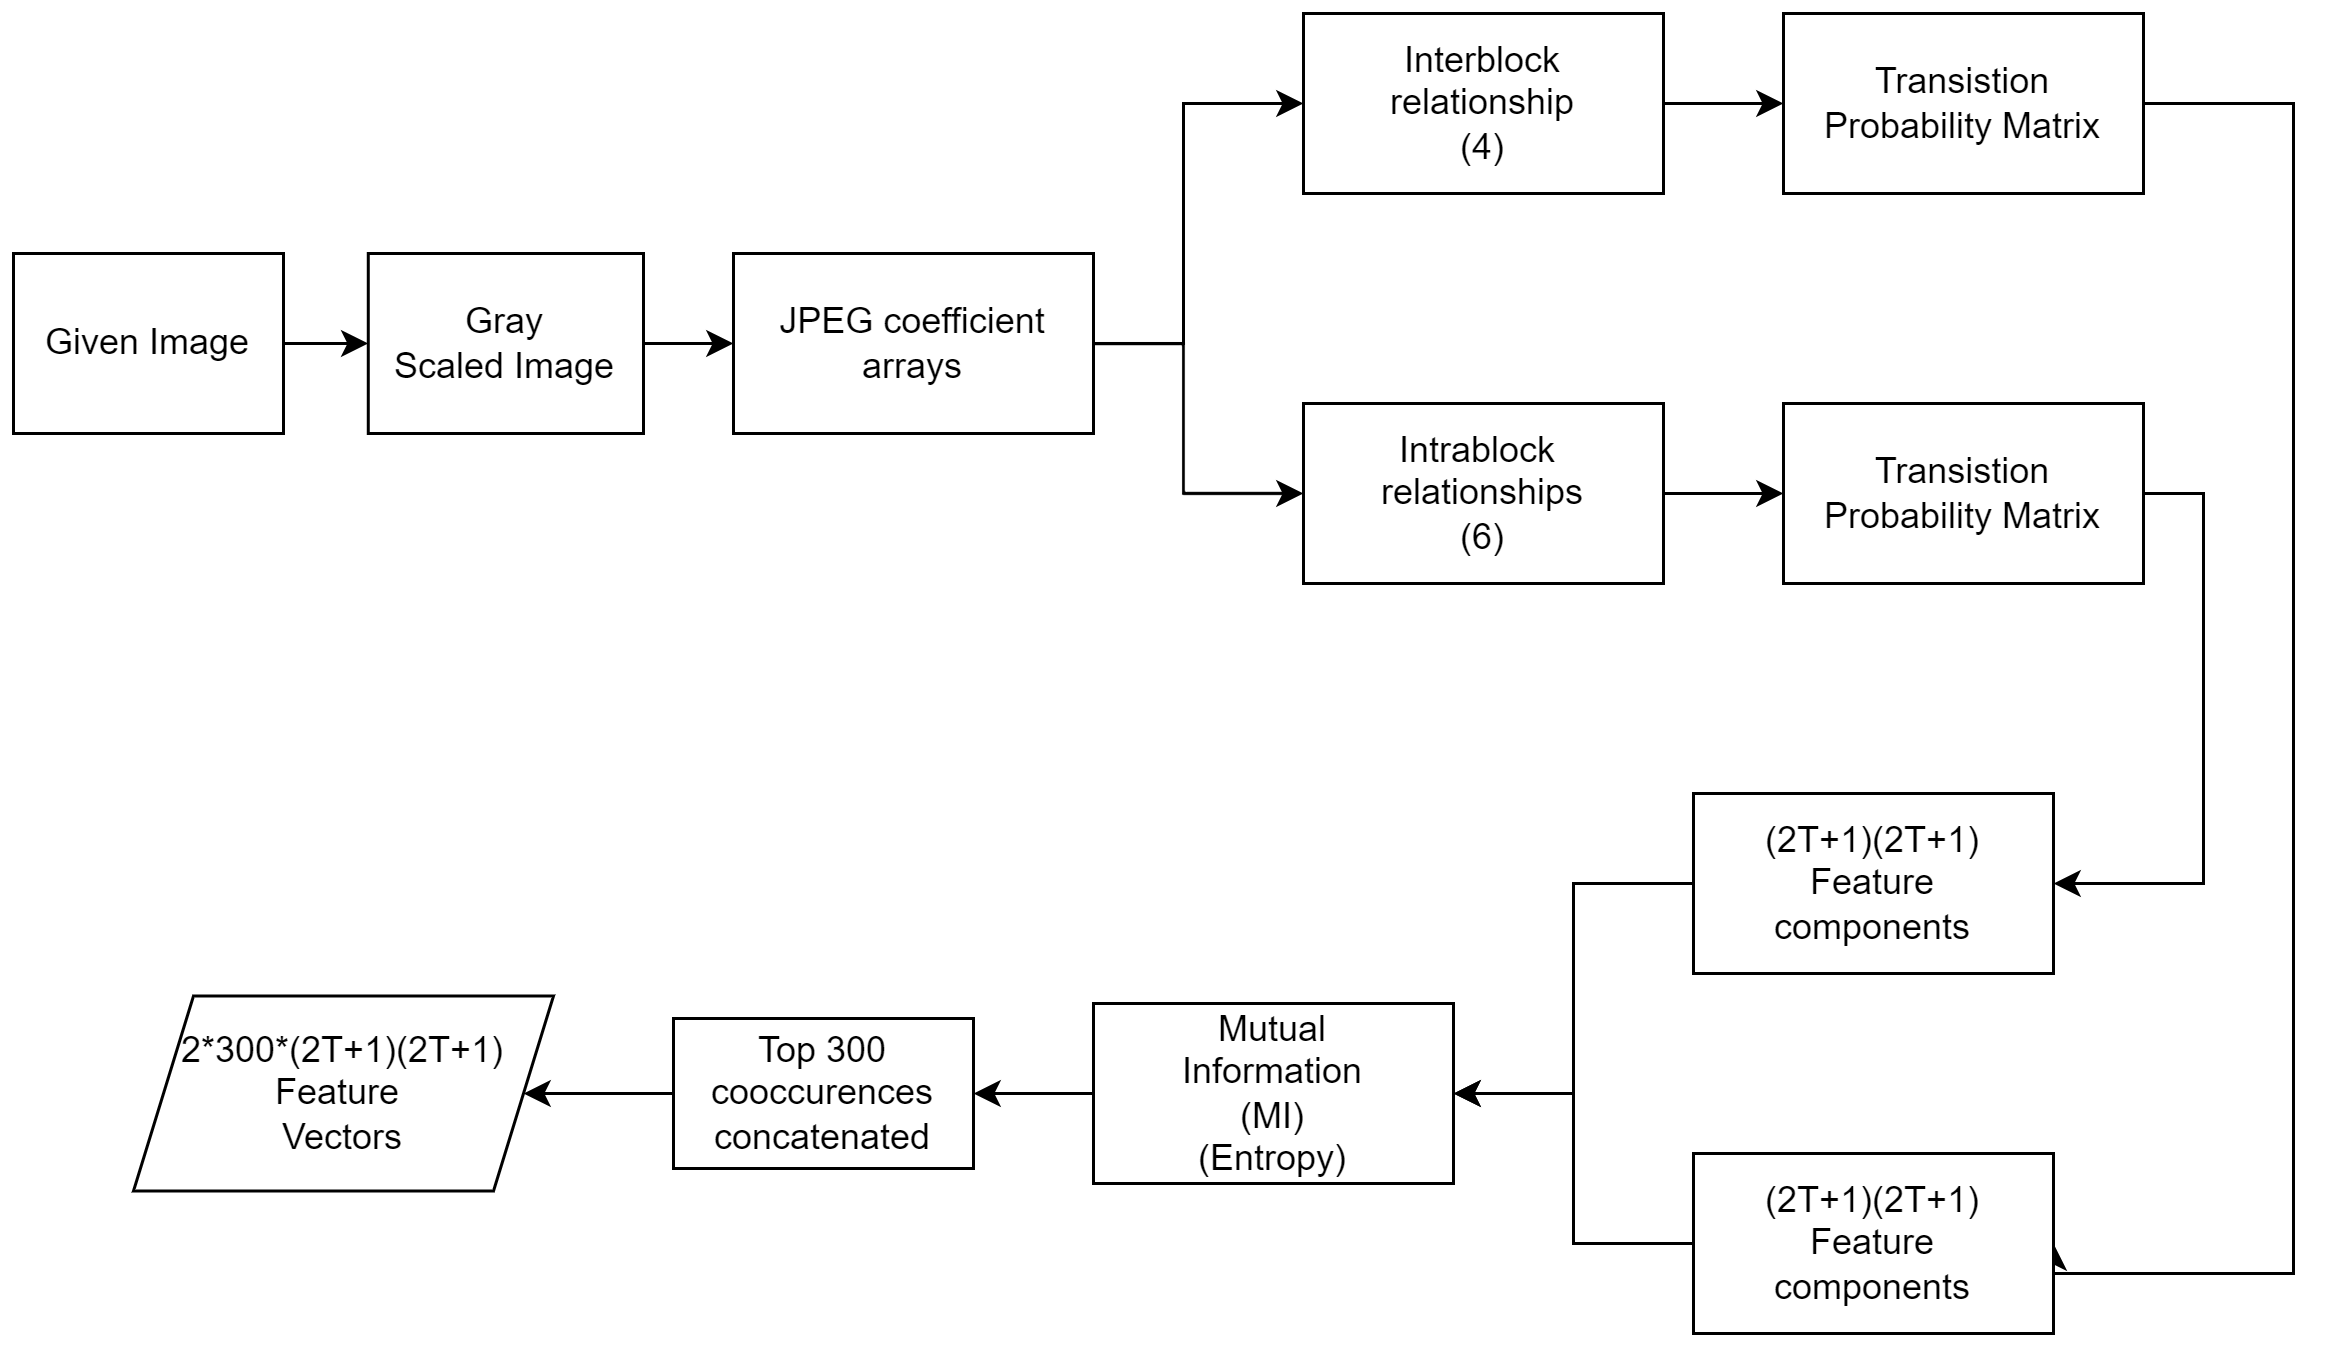
\includegraphics[width=150mm]{./img/feature_extraction.png}
    \caption{Feature Extraction Process}
\end{figure}

\section{Ensemble Classifiers}
Ensemble classifiers are machine learning techniques that combine multiple individual models, or ``base learners,'' to make predictions. The main idea behind the ensemble methodology is to weigh several individual classifiers, and combine them in order to obtain a classifier that outperforms every one of them. The key objective of the ensemble methods is to reduce bias and variance. High bias means the model is too simplistic and may not capture the underlying patterns in the data, leading to underfitting. Ensemble methods aim to reduce bias by combining multiple models, each capturing different aspects of the data. High variance means the model is overly complex and may capture noise or random fluctuations in the data, leading to overfitting. Ensemble methods aim to reduce variance by averaging the predictions of multiple models, smoothing out individual fluctuations and creating a more stable and reliable overall prediction.\\
Some of widely used ensemble methods are:
\begin{itemize}[noitemsep]
    \item \textbf{Bagging:} Bagging, or Bootstrap Aggregating, is an ensemble method that involves training multiple models on different subsets of the training data and combining their predictions. The subsets are created by sampling the training data with replacement, and each model is trained on a different subset. The final prediction is made by averaging the predictions of all the models. Bagging helps reduce variance by creating diverse models and averaging their predictions, leading to a more stable and reliable overall prediction.
    \begin{figure}[H]
        \centering
        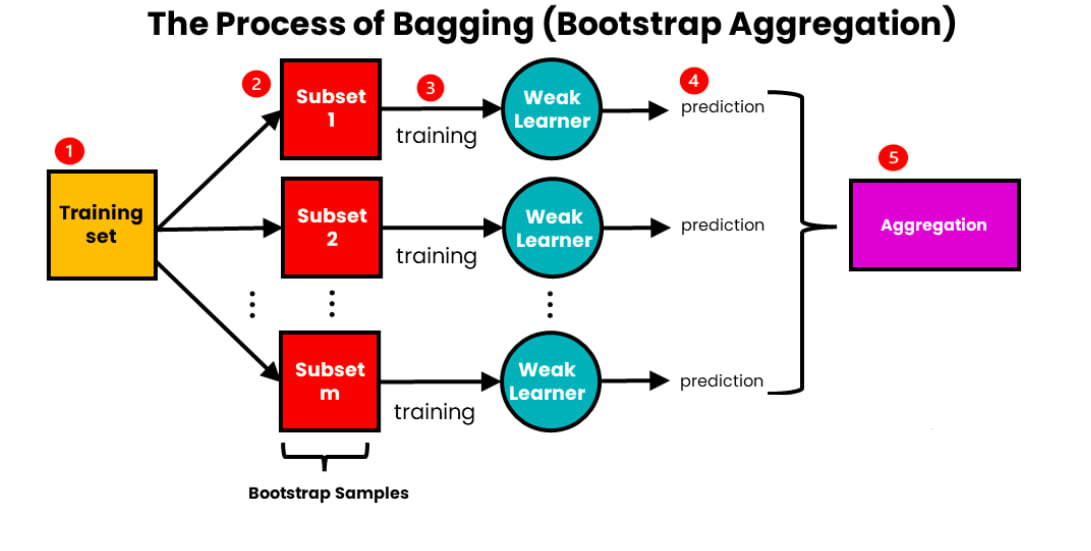
\includegraphics[width=120mm]{./img/bagging.jpg}
        \caption*{\small{\textit{Source: https://www.analyticsvidhya.com/blog/2023/01/ensemble-learning-methods-bagging-boosting-and-stacking/}}}
        \caption{Basic outline of Ensemble Classifier}
    \end{figure}
    \item \textbf{Boosting:} Boosting is an ensemble method that involves training multiple models sequentially, with each model learning from the mistakes of the previous models. The final prediction is made by combining the predictions of all the models. Boosting helps reduce bias by focusing on the mistakes made by the previous models and learning from them.
    \begin{figure}[H]
        \centering
        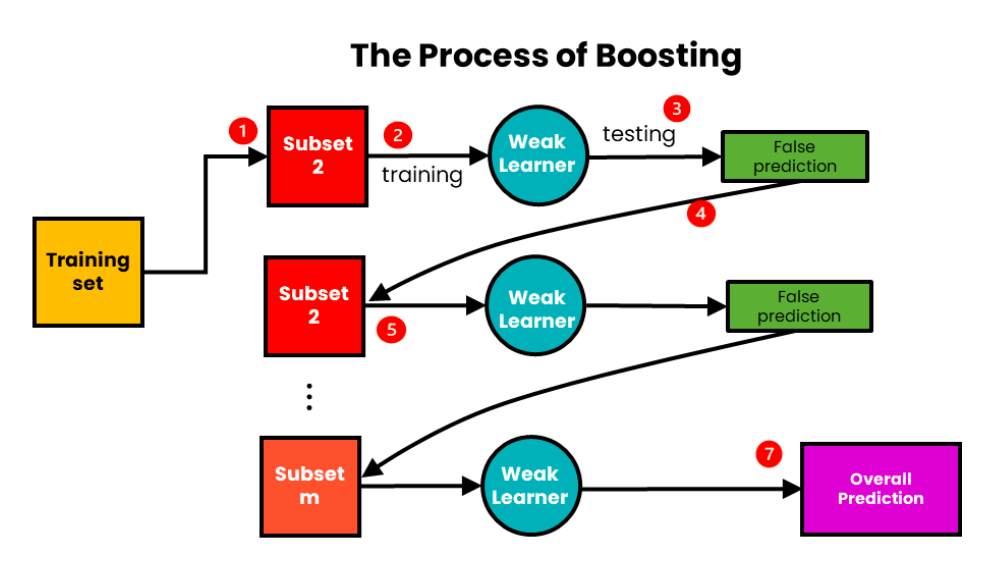
\includegraphics[width=120mm]{./img/boosting.png}
        \caption*{\small{\textit{Source: https://www.analyticsvidhya.com/blog/2023/01/ensemble-learning-methods-bagging-boosting-and-stacking/}}}
        \caption{Basic outline of Boosting Classifier}
    \end{figure}
    \item \textbf{Stacking:} Stacking is an ensemble method that involves training multiple models and combining their predictions using another model, called a meta-learner. The meta-learner is trained on the predictions of the base models and learns to combine them into a final prediction.
    \begin{figure}[H]
        \centering
        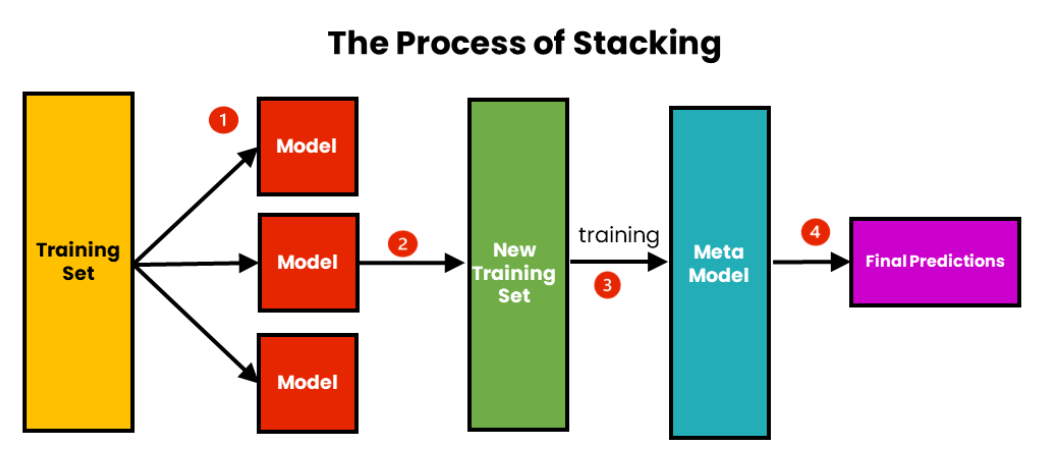
\includegraphics[width=120mm]{./img/Stacking.png}
        \caption*{\small{\textit{Source: https://www.analyticsvidhya.com/blog/2023/01/ensemble-learning-methods-bagging-boosting-and-stacking/}}}
        \caption{Basic outline of Stacking Classifier}
    \end{figure}
\end{itemize}
A standard ensemble approach used in classification tasks consists of the following fundamental components:
\begin{enumerate}
    \item \textbf{Training set:} A labeled dataset is used for ensemble training. The instances of the dataset are described as attribute-value vectors. This set is crucial as it serves as the foundation for training the ensemble model, providing the necessary data points and their corresponding labels. In other words, it's the collection of data points used to train an ensemble learning algorithm. Each data point in the training set consists of two parts: the features (or attributes) and the label (or output). The features are the input variables used to predict the label, and the label is the output variable we want to predict.
    \item \textbf{Base Inducer:} The inducer is an induction algorithm that obtains a training set and forms a classifier that represents the generalized relationship between the input attributes and the target attribute. Decision trees, Neural networks, Support Vector Machines(SVMs), k-Nearest Neighbors(k-NN), Random Forsets, Gradient Boosting Machines(GBMs), AdaBoost etc. are different types of base learners that can be used in ensemble methods. The choice of base learner plays a vital role in the ensemble's performance and is often selected based on the nature of the problem and the characteristics of the data.
    \item \textbf{Diversity Generator:}This component is responsible for generating the diverse classifiers. Diversity among the classifiers is crucial as it helps improve the ensemble's performance by ensuring that the individual models provide different perspectives on the data. Techniques such as bagging, boosting, and randomization can be used to generate diverse classifiers.
    \item \textbf{Combiner:} The combiner is responsible for combining the classifications of the various classifiers. Some of the widely used combination methods are Weighting method, Majority voting, Performance weighting, Distribution summation, Bayesian combination, Dempster-Shafter, Vogging, Naive bayes. The choice of combination method depends on the nature of the problem and the characteristics of the data. The combiner's role is to aggregate the predictions of the individual models to produce the final ensemble prediction, which often leads to improved overall performance compared to using a single model.\cite{21} 
\end{enumerate}

\subsection{Algorithm}
\begin{algorithm}[H]
    \caption{Ensemble Classifier Algorithm \cite{5}}
    \begin{algorithmic}[1]
    \For{$l=1$ to $L$}
        \State Form a random subspace
        \State $D_l \subset \{1, \dots, d\}, \lvert D_l \rvert = d_{\text{sub}} < d$
        \State Form a bootstrap sample $N_1^b$, $\lvert N_1^b \rvert = N^{\text{trn}}$ by uniform sampling with \mbox{replacement} from the set $\{1, \dots, N^{\text{trn}}\}$
        \State Train a base learner $B_l$ on features
        \State $X_l = \{x_m^{(D_l)}, \bar{x}_m^{(D_l)}\}_{m \in N_l^b}$
        \State $\rightarrow$ obtain eigenvector $v_l$ and threshold $T_l$
    \EndFor
    \ForAll{$y \in Y^{\text{tst}}$}
        \For{$l=1$ to $L$}
            \State Make $l^{th}$ decision: $B_l(y^{D_l}) \triangleq \begin{cases} 1, & \text{when } v_l^Ty^{(D_l)} > T_l \\ 0, & \text{otherwise} \end{cases}$
        \EndFor
    \EndFor
    \State Form the final decisions $B(y)$ by majority voting: \\
    $B(y) = \begin{cases} 1, & \text{when } \sum_{l=1}^{L} B_l(y^{(D_l)}) > L/2 \\ 0, & \text{when } \sum_{l=1}^{L} B_l(y^{(D_l)}) < L/2 \end{cases}$
    \State \textbf{return} $B(y)$, $y \in Y^{\text{tst}}$
    \end{algorithmic}
    \end{algorithm}
    \begin{flushleft}
    In the provided algorithm:\\
    \end{flushleft}
     $d$: Represents the dimensionality of the feature space.\\
     $d_{\text{sub}}$: Represents the dimensionality of the feature subset.\\
     $N^{\text{TRN}}$ and $N^{\text{TST}}$: Denote the number of training and testing examples, respectively.\\
     $L$: Represents the number of base learners.\\
     $x_m, \bar{x}_m \in \mathbb{R}^d, m=1,...,N^{\text{TRN}}$: Refer to the cover and stego features computed from the training set.\\
     $y_k, \bar{y}_k \in \mathbb{R}^d, k=1,...,N^{\text{TST}}$: Denote the cover and stego features computed from the testing set.\\
\clearpage
\section{Model Training Approach}
\textbf{Ensemble Classifier Selection:}\\
The decision for selecting an ensemble classification approach is based on the problem at hand. The bagging approach appears ideal for this classification problem as it effectively addresses issues such as overfitting, prevalent during model training. One of the main focuses of our model is diversity, and bagging achieves this by creating diverse bootstrapped samples, enhancing the accuracy of the classification. Bagging also allows parallelization, significantly reducing training time compared to other models like boosted ensemble classifiers, L-SVM, or G-SVM. The simplicity and instability of bagging contribute to its advantages for ensemble classification.\vspace{0.25cm}\\
\textbf{Bootstrapping:}\\
Bootstrapping is simply the process of randomly dividing the dataset into various parts and feeding them to the number of base learners present inside the ensemble classifier for training. The datasets are divided into various smaller samples and then sent to the base learners for training. This division of datasets removes their dependency on each other, promoting parallelization and allowing the training of various models simultaneously..\vspace{0.25cm}\\
\textbf{Base Learner Training:}\\
The base learners are fed with the feature "dsub," a subset of "d" where "d" is the total number of features or dimensions of each data. The base learners are trained on Fisher's Linear Discriminant Analysis (FLD), which outputs binary classification. FLD is chosen for its diversity in revealing various errors, increasing the diversity of each base learner and resulting in a more accurate ensemble classifier.\vspace{0.25cm}\\
\textbf{Aggregation:}\\
The trained model can now successfully classify the input images as cover or steganographically modified images. The binary classifier typically classifies 1 as a steganographically modified image and 0 as a cover image. The chosen voting method is hard voting, which calculates the number of 0s and 1s and outputs the result dominated by the majority. The threshold is set at L/2.
\vspace{0.25cm}\\
\textbf{Efficiency Considerations:}\\
The system prioritizes efficiency by embracing shallow machine learning techniques, specifically ensemble classifiers, instead of deep learning approaches. This strategic choice aligns with the computational efficiency goal, ensuring effective steganalysis without the computational demands associated with deep learning architectures. The intentional selection of CC-C300 as a feature further amplifies efficiency and bolsters the system's detection capabilities. This streamlined approach aims to strike a balance between accuracy and efficiency in steganalysis.\\
\clearpage
\section{FLD as Base Learner}
Fisher's Linear Discriminant (FLD), also known as Linear Discriminant Analysis (LDA), is a popular method used for dimensionality reduction and classification. It was introduced by Ronald A. Fisher in 1936 and is based on the idea of finding a linear combination of features that characterizes or separates two or more classes of objects or events. FLD is a supervised learning algorithm, meaning it requires labeled data to train the model. It is commonly used for classification tasks, where the goal is to predict the class label of a new data point based on its features. FLD works by finding the linear combination of features that maximizes the separation between the classes while minimizing the variation within each class. This linear combination is known as the discriminant function, and it is used to classify new data points. FLD is particularly effective when the number of features is larger than the number of samples. FLD is widely used in various fields, including pattern recognition, machine learning, and statistics, and it has been successfully applied to a wide range of classification problems.
\\
Modern steganographic methods typically require a high dimensional feature representation of images for accurate detection. FLD is well-suited for this task and is a widely used machine learning tool for steganalysis of digital media due to its efficiency when working with high dimensional feature sets. It is also known for its ability to handle multicollinearity, a common issue in high dimensional feature sets.\cite{23}\\
\subsection{FLD algorithm for Image steganalysis} 
\begin{enumerate}[noitemsep]
    \item \textbf{Input:}
    \begin{itemize}
        \item Training sets of cover and stego image features (matrices of size \(d \times N_{\text{trn}}\))
        \item Number of base learners (\(L\))
        \item Dimensionality of the feature space (\(d\))
        \item Number of features selected for each base learner (\(d_{\text{sub}}\))
    \end{itemize}
    
    \item \textbf{Calculate the means (\( \mu_c \) and \( \mu_s \)) and covariance matrices (\( \Sigma_c \) and \( \Sigma_s \)) of the cover and stego image features.}
    
    \item \textbf{For each base learner:}
    \begin{itemize}
        \item[a.] Randomly select \(d_{\text{sub}}\)-dimensional subsets of the feature space.
        \item[b.] Calculate the weighting vector (\(w\)) using the Fisher Linear Discriminant (FLD) criterion:
        \begin{itemize}
            \item Calculate the means (\( \mu_c \) and \( \mu_s \)) and covariance matrices (\( \Sigma_c \) and \( \Sigma_s \)) for the selected features.
            \item Calculate the weighting vector (\(w\)) using the formula: \(w = (\Sigma_c + \Sigma_s)^{-1} (\mu_c - \mu_s)\)
        \end{itemize}
    \end{itemize}
    
    \item \textbf{Combine the decisions of all base learners:}
    \begin{itemize}
        \item[a.] For each test feature vector (\(f\)):
        \begin{itemize}
            \item Calculate the projections (\(v\)) of the feature vector onto the weighting vectors of all base learners.
            \item Combine the decisions of all base learners using a majority voting rule or other fusion method.
        \end{itemize}
    \end{itemize}
    
    \item \textbf{Output:} The final classification decision for the test feature vector.
\end{enumerate}

\subsection{Mathematics}

\begin{itemize}[leftmargin=*]
    \item \textbf{Class Mean:}
    \begin{itemize}
        \item Calculate the mean vectors for each class:
        \begin{align*}
            m_1 &= \frac{1}{N_1} \sum_{i=1}^{N_1} x_i^{(1)} \\
            m_2 &= \frac{1}{N_2} \sum_{i=1}^{N_2} x_i^{(2)}
        \end{align*}
        Where \(N_1\) and \(N_2\) are the number of samples in class \(C_1\) and \(C_2\) respectively, and \(x_i^{(1)}\) and \(x_i^{(2)}\) are feature vectors for individual samples.
    \end{itemize}
    
    \item \textbf{Within-Class Scatter Matrix:}
    \begin{itemize}
        \item Calculate the within-class scatter matrix \(S_w\):
        \[ S_w = \sum_{i=1}^{N_1} (x_i^{(1)} - m_1)(x_i^{(1)} - m_1)^T + \sum_{i=1}^{N_2} (x_i^{(2)} - m_2)(x_i^{(2)} - m_2)^T \]
    \end{itemize}
    
    \item \textbf{Between-Class Scatter Matrix:}
    \begin{itemize}
        \item Calculate the between-class scatter matrix \(S_b\):
        \[ S_b = (m_1 - m_2)(m_1 - m_2)^T \]
    \end{itemize}
    
    \item \textbf{Fisher's Criterion:}
    \begin{itemize}
        \item Find the optimal weight vector \(W\) by maximizing the Fisher's criterion:
        \[ W = S_w^{-1} (m_1 - m_2) \]
        Where \(S_w^{-1}\) is the inverse of the within-class scatter matrix.
    \end{itemize}
    
    \item \textbf{Decision Rule:}
    \begin{itemize}
        \item The decision rule for classifying a new feature vector \(x\) is determined by:
        \begin{align*}
            &\text{if } W^T x > \text{Threshold}, \text{ then classify as } C_1 \\
            &\text{if } W^T x \leq \text{Threshold}, \text{ then classify as } C_2
        \end{align*}
    \end{itemize}
\end{itemize}

\clearpage 

